\subsection{Caso d'uso UC5: Esportazione della presentazione}
	\begin{figure}[h] 
		\centering 
		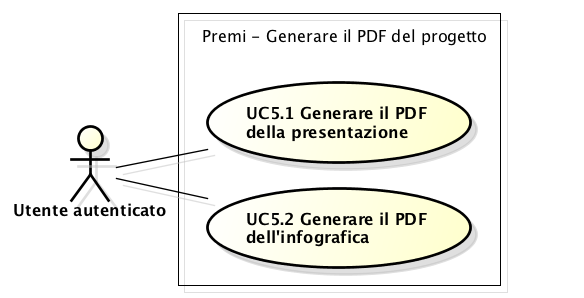
\includegraphics[scale=0.45] {img/UC5.png} 
		\caption{UC5 - Esportazione della presentazione} 
	\end{figure}
	
	\begin{itemize}
		\item \textbf{Attori:} Utente;
		\item \textbf{Scopo e descrizione:} L'utente ha creato una presentazione di slide e vuole esportarla in un formato diverso per salvarla nel proprio computer;
		\item \textbf{Precondizione:} Il sistema è in attesa che l'utente selezione la funzione esporta presentazione;
		\item \textbf{Flusso degli eventi:}
		\begin{enumerate}
			\item L'utente seleziona dal menù la funzione esporta [UC5.1];
			\item L'utente sceglie il formato in cui esportare la presentazione [UC5.2];
			\item L'utente sceglie dove esportare la presentazione [UC5.3];
			\item L'utente conferma l'esportazione [UC5.4];
		\end{enumerate}
		\item \textbf{Postcondizione:} Il sistema ha esportato la presentazione.
	\end{itemize}


\subsection{Caso d'uso UC5.1: Selezionare funzione esporta}
	\begin{itemize}
		\item \textbf{Attori:} Utente;
		\item \textbf{Scopo e descrizione:} L'utente seleziona dal menù la funzione esporta per esportare la presentazione;
		\item \textbf{Precondizione:} Il sistema è in attesa che l'utente selezioni la funzione dal menù;
		\item \textbf{Postcondizione:} Il sistema apre la finestra di dialogo per l'esportazione.
	\end{itemize}


\subsection{Caso d'uso UC5.2: Selezionare il formato di esportazione}
	\begin{itemize}
		\item \textbf{Attori:} Utente;
		\item \textbf{Scopo e descrizione:} L'utente deve scegliere il formato in cui esportare la presentazione;
		\item \textbf{Precondizione:} Il sistema è in attesa che l'utente selezioni il formato dall'apposita finestra di dialogo;
		\item \textbf{Postcondizione:} Il sistema registra la scelta e apre la finestra di dialogo per il salvataggio della presentazione esportata.
	\end{itemize}


\subsection{Caso d'uso UC5.3: Selezionare la destinazione di esportazione}
	\begin{itemize}
		\item \textbf{Attori:} Utente;
		\item \textbf{Scopo e descrizione:} L'utente deve scegliere la destinazione in cui salvare la presentazione esportata.
		\item \textbf{Precondizione:} Il sistema è in attesa che l'utente selezioni il percorso dall'apposita finestra di dialogo;
		\item \textbf{Postcondizione:} Il sistema registra la destinazione desiderata.
	\end{itemize}


\subsection{Caso d'uso UC5.4: Confermare l'esportazione}
	\begin{itemize}
		\item \textbf{Attori:} Utente;
		\item \textbf{Scopo e descrizione:} L'utente deve confermare l'esportazione della presentazione nel formato e nella destinazione desiderata;
		\item \textbf{Precondizione:} Il sistema è in attesa che l'utente confermi l'esportazione;
		\item \textbf{Postcondizione:} Il sistema ha esportato la presentazione.
	\end{itemize}
	
	
\subsection{Caso d'uso UC5.5: Selezionare il percorso}
	\begin{figure}[h] 
		\centering 
		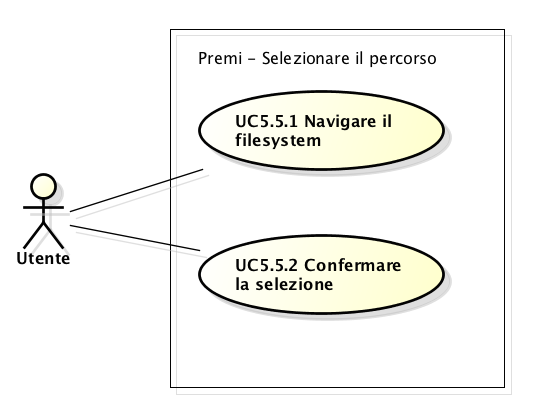
\includegraphics[scale=0.45] {img/UC5.5.png} 
		\caption{UC5.5 - Selezionare la destinazione} 
	\end{figure}
	\begin{itemize}
		\item \textbf{Attori:} Utente;
		\item \textbf{Scopo e descrizione:} L'utente deve scegliere il percorso. Naviga il filesystem, lo seleziona ne e conferma la scelta;
		\item \textbf{Precondizione:} Il sistema è in attesa che l'utente navighi il filesystem e confermi il percorso scelto;
		\item \textbf{Flusso degli eventi:}
		\begin{enumerate}
			\item L'utente naviga il filesystem alla ricerca della posizione desiderata [UC5.5.1];
			\item L'utente conferma la posizione selezionata [UC5.5.2].
		\end{enumerate}
		\item \textbf{Postcondizione:} Il sistema registra il percorso desiderato.
	\end{itemize}
	
	\subsection{Caso d'uso UC5.5.1: Navigare il filesystem}
	\begin{itemize}
		\item \textbf{Attori:} Utente;
		\item \textbf{Scopo e descrizione:} L'utente può navigare il filesystem per selezionare la cartella dentro la quale vuole esportare la presentazione;
		\item \textbf{Precondizione:} Il sistema è in attesa che l'utente selezioni una cartella;
		\item \textbf{Postcondizione:} Il sistema ha aggiornato la il percorso con quello scelto dall'utente.
	\end{itemize}
	
	\subsection{Caso d'uso UC5.5.2: Confermare selezione}
	\begin{itemize}
		\item \textbf{Attori:} Utente;
		\item \textbf{Scopo e descrizione:} L'utente conferma che il percorso selezionato è quello corretto;
		\item \textbf{Precondizione:} Il sistema ha selezionato il percorso indicato dall'utente;
		\item \textbf{Postcondizione:} Il sistema ha registrato il percorso precedentemente scelto dall'utente.
	\end{itemize}